\subsection{Questão de Pesquisa 4}

\emph{Qual o foco da contribuição de pesquisa realizada em SOC e relacionada com qualidade de serviço? }

Com o intuito de responder a esta questão, foi feita uma avalia\c c\~{a}o da distribui\c c\~{a}o dos 
artigos em rela\c c\~{a}o ao tipo de pesquisa (conforme discutido na Se\c c\~{a}o~\ref{sec:review_method}). 
O \emph{bubble plot} na Figura~\ref{fig:bubbleplot-QoSRes}  apresenta tal distibui\c c\~{a}o, novamente sendo importante ressaltar que o n\'{u}mero total de artigos nos gr\'{a}ficos \'{e} superior ao n\'{u}mero total de artigos analisados--- uma vez que alguns artigos apresentam contribui\c c\~{o}es tanto em termos de uma nova solu\c c\~{a}o proposta quanto em termos de avalia\c c\~{a}o e/ou valida\c c\~{a}o. Por exemplo, Huang et al. prop\~{o}e um modelo estoc\'{a}stico para representar e raciocinar sobre dependabilidade em um ambiente de SOC, ao mesmo tempo que valida formalmente tal proposta por meio de provas de teoremas~\cite{huang:scc2011}.

\begin{figure}[htb]
\centering
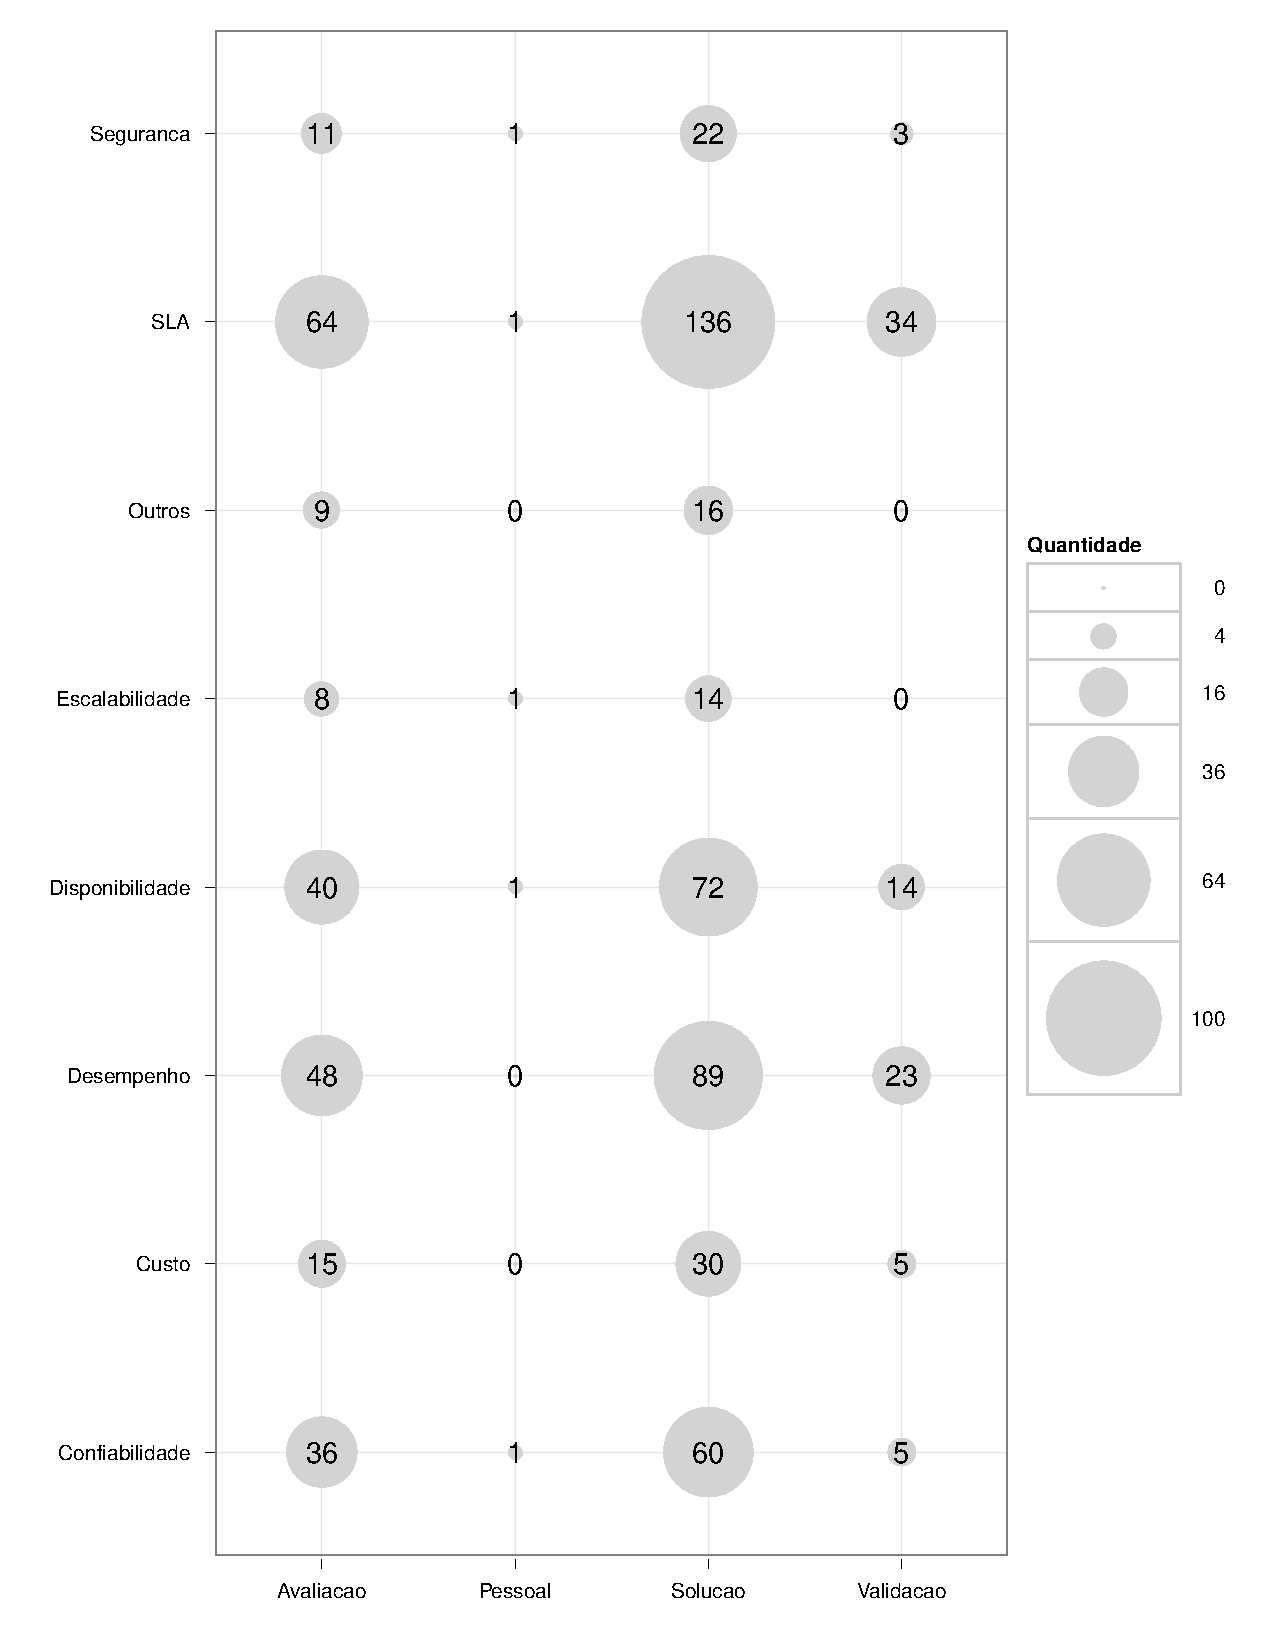
\includegraphics[scale=0.5]{imagens/pesquisaContexto.pdf}
\caption{\emph{Bubble plot} com a distribui\c{c}\~{a}o envolvendo Tipo de Pesquisa e Contexto}
\label{fig:bubbleplot-QoSRes}
\end{figure}

Esta investiga\c c\~{a}o revelou que 21 artigos (como por exemplo~\cite{jeong:fqs2009,ardagna:jss2010}) 
contribuem com uma nova solu\c c\~{a}o para lidar com qualidade de servi\c co em SOC ao mesmo tempo que apresentam uma investiga\c c\~{a}o tanto em termos de avalia\c c\~{a}o quanto em termos de valida\c c\~{a}o. Al\'{e}m disso, 80 artigos s\~{a}o propostas de solu\c c\~{o}es que apresentam avalia\c c\~{o}es em termos de estudos de casos mais simples, n\~{a}o compreendendo uma valida\c c\~{a}o da(s) t\'{e}cnica(s) proposta(s). Entre esses artigos podemos citar~\cite{filieri:faa2012,nascimento:splc2011}. Finalmente, 27 artigos apresentam, al\'{e}m de uma nova solu\c c\~{a}o relacionada \`{a} qualidade de servi\c cos em SOC, uma s\'{o}lida valida\c c\~{a}o (e.g.~\cite{huang:scc2011,binshtok:icsoc2009}). Por outro lado, 102 artigos (aproximadamente 40\% do total) prop\~{o}em novas solu\c c\~{o}es sem apresentar avalia\c c\~{a}o ou valida\c c\~{a}o consistentes (\cite{balfagih:icime2011}). Enquanto que apenas 4 artigos focam na avalia\c c\~{a}o e/ou valida\c c\~{a}o de propostas existentes~\cite{voelz:edoc2010,moayed:icsea2010}.  

Esses n\'{u}meros revelam que a \'{a}rea de pesquisa de qualidade de servi\c co em SOC ainda est\'{a} em uma fase de amadurecimento, onde um percentual significativo das contribui\c c\~{o}es simplesmente apresentam novas abordagens ou fazem compara\c c\~{o}es envolvendo a pr\'{o}pria t\'{e}cnica proposta--- o que pode levar a conclus\~{o}es tendenciosas. A quantidade de artigos que visam avaliar ou validar t\'{e}cnicas existentes, algo recomendado antes de se iniciar a concep\c c\~{a}o de uma nova solu\c c\~{a}o, \'{e} praticamente insignificante. 